%-------------------------------------------------------------------------------
% menu
%-------------------------------------------------------------------------------
%
% \file        menu.tex
% \library     Documents
% \author      Chris Ahlstrom
% \date        2015-08-31
% \update      2020-12-30
% \version     $Revision$
% \license     $XPC_GPL_LICENSE$
%
%     Provides the Menu section of seq66-user-manual.tex.
%
%-------------------------------------------------------------------------------

\section{Menu}
\label{sec:menu}

   The \textsl{Seq66} menu structure is more complex than
   that of \textsl{Seq24}.  In particular, the \textsl{File} menu has two
   variants:  a normal file menu, and a file menu when \textsl{Seq66} is
   running under the \textsl{Non Session Manager}.

\subsection{Menu / File}
\label{subsec:menu_file}

   The \textbf{File} menu is used to save and load files in
   Standard MIDI Format 0 or 1, \textsl{Cakewalk} "WRK",
   and \textsl{Seq66} MIDI files.
   The \textsl{Seq66} menu entry contains the sub-items shown below.
%  \figureref{fig:menu_file_items}.
   The next few sub-sections discuss
   the sub-items in the \textbf{File} menu.
   Please note that these entries are different
   if \textsl{Seq66} is start under the control of the
   \textsl{Non Session Manager}.  

\begin{figure}[H]
   \centering 
   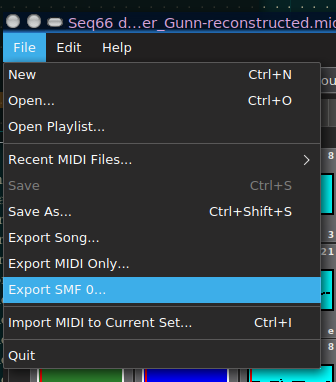
\includegraphics[scale=0.75]{main-menu/file/livegrid-dark-menu-file.png}
   \caption{Seq66 Menu File Items}
   \label{fig:menu_file_items}
\end{figure}

   \begin{enumber}
      \item \textbf{New}
      \item \textbf{Open}
      \item \textbf{Open Playlist}
      \item \textbf{Recent MIDI files}
      \item \textbf{Save}
      \item \textbf{Save As}
      \item \textbf{Export Song as MIDI}
      \item \textbf{Export MIDI Only}
      \item \textbf{Import MIDI to Current Set}
      \item \textbf{Quit} (\textbf{Exit} in \textsl{Windows})
   \end{enumber}

   For information on the \textbf{File} menu when \textsl{Seq66} is
   running under the \textsl{Non Session Manager}, see
   \sectionref{subsubsec:sessions_file_menu}.

\subsection{Menu / File / New}
\label{subsec:menu_file_new}

   The \textbf{New} menu entry clears the current song.
   (A play-list or mute-groups setup, if loaded, are not affected.)
   If unsaved changes are pending, the user is prompted to save the changes.
   Prompting for changes is more comprehensive than \textsl{Seq24}.
   However, when in doubt, save!
   Keep backups of your tunes and configuration files!

\subsubsection{Menu / File / Open}
\label{subsubsec:menu_file_open}

   The \textbf{Open} menu entry opens a song (MIDI file or \textsl{Cakewalk}
   WRK file), replacing the current song (after a prompt if the song was
   modified).
   It opens up a standard file dialog:

\begin{figure}[H]
   \centering 
   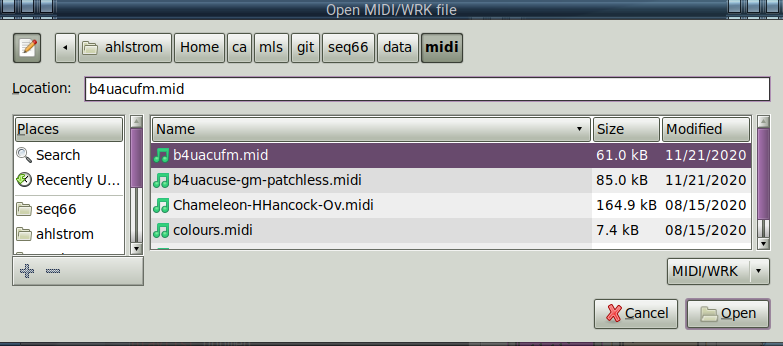
\includegraphics[scale=0.65]{main-menu/file/light-menu-file-open.png}
   \caption{File / Open}
   \label{fig:menu_file_open}
\end{figure}

   This dialog lets one type a file-name, highlighting the first file
   that matches the characters typed.
   \textsl{Seq66} can open \textsl{Seq66}, regular MIDI files, and
   \textsl{Cakewalk} "WRK" files.

\subsubsection{Menu / File / Open Playlist}
\label{subsubsec:menu_file_open_playlist}

   The \textbf{Open Playlist...} menu entry opens a \textsl{Seq66}
   play-list file.

\begin{figure}[H]
   \centering 
   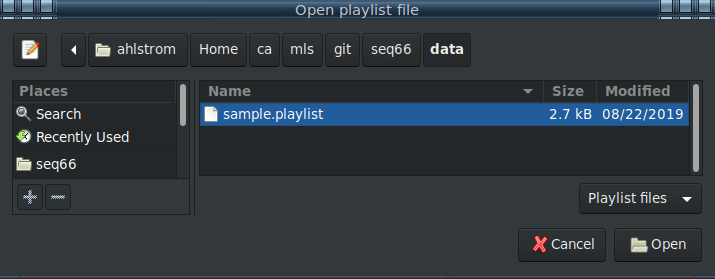
\includegraphics[scale=0.65]{main-menu/file/dark-menu-file-open-playlist.png}
   \caption{File / Open Playlist}
   \label{fig:menu_file_open_playlist}
\end{figure}

   The playlist file contains a list of "playlist sections",
   each listing a number of MIDI songs.
   These playlists and songs can be
   selected by the arrow keys or by MIDI control,
   and are displaed and editiable in the \textsl{Playlist} tab
   in the main window.
   See \sectionref{sec:playlist}.

\subsubsection{Menu / File / Recent MIDI files}
\label{subsubsec:menu_file_recent}

   This menu entry provides a list of the last few MIDI files created or opened;
   play-list selections are \textsl{not} included in this list.

\begin{figure}[H]
   \centering 
   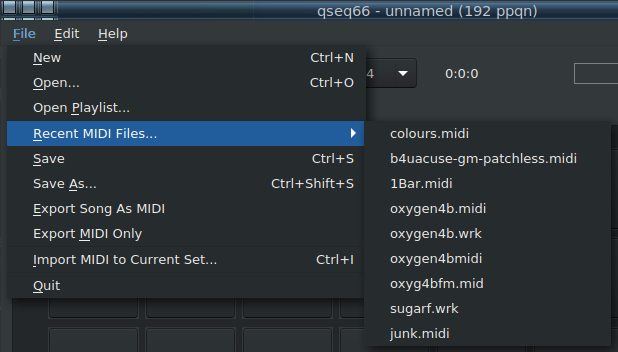
\includegraphics[scale=0.65]{main-menu/file/dark-menu-recent-files.png}
   \caption{Seq66 Menu File Recent Files}
   \label{fig:menu_file_recent_files}
\end{figure}

   This list is saved in the \texttt{[recent-files]} section of the
   'rc' configuration file.
   In the menu, only the last part of the file-name is
   shown, but in the 'rc' file,
   the full path to the file-name is stored.
   This path is in "UNIX" format, using the forward slash, or solidus,
   as the path separator, even in \textsl{Windows}.
   Only unique entries are included in the recent-files list.
   The limit is 10 recent-file entries.
   This is a feature from \textsl{Kepler34} \cite{kepler34}.
   One can also set \textsl{Seq66} to load the most-recent file at startup.
   Here is an example from an 'rc' file.  Note the startup option.

\begin{verbatim}
   [recent-files]
   # Holds a list of the last few recently-loaded MIDI files.
   # The first number is the number of items in the list.  The second value
   # indicates if to load the most recent file (the top of the list)
   # at startup (1 == load it).
   3 1
   /home/chris/git/seq66/data/b4uacuse-gm-patchless.midi
   /home/chris/git/seq66/data/midi/colours.midi
   /home/chris/git/Julian-data/TestBeeps.midi
\end{verbatim}

\subsubsection{Menu / File / Save and Save As}
\label{subsubsec:menu_file_open_save_as}

   The \textbf{Save} menu entry saves the song under its current file-name.
   If there is no current file-name, it opens up a standard file
   dialog to name and save the file.
   The \textbf{Save As} menu entry saves a song under a different name.
   It opens up the following standard file dialog, very similar to the 
   \textbf{File Open} dialog, with an additional \textbf{Name} text-edit field.

\begin{figure}[H]
   \centering 
   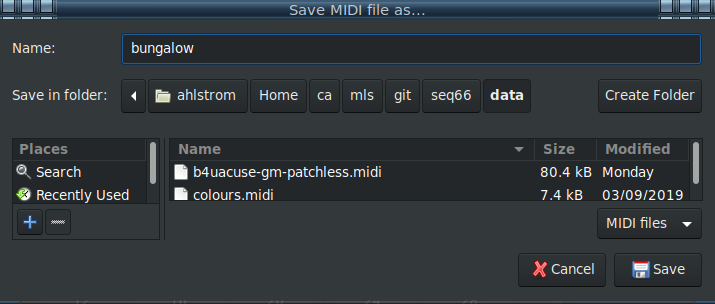
\includegraphics[scale=0.65]{main-menu/file/dark-menu-file-save-as.png}
   \caption{File / Save As}
   \label{fig:menu_file_save_as}
\end{figure}

   To save a new file or save the current file to a new name,
   enter the name in the name field, without an extension.
   \textsl{Seq66} will append a \texttt{.midi} extension to the filename.
   The file will be saved in a format that the Linux \textsl{file} command
   will tag as something like:

   \begin{verbatim}
      colours.midi: Standard MIDI data (format 1) using 16 tracks at 1/192
   \end{verbatim}

   It looks like a simple MIDI file, and yet, if one re-opens it in
   \textsl{Seq66}, one sees that the mute-groups, labeling, pattern
   information, and song layout have been preserved in this file.
   This information is saved in a way that MIDI-compliant software
   should be able to use or ignore without failure.
   After the last track in the file, a number of
   \index{SeqSpec}
   sequencer-specific (SeqSpec) items are saved, to preserve
   the extra information that \textsl{Seq66} adds to the song.
   There is no way to save a \textsl{Cakewalk} "WRK" file.
   \textsl{Seq66} can only read them, and then save them as
   \textsl{Seq66} files.

   \index{Meta events}
   Meta events are now partially handled by \textsl{Seq66}.
   Meta events \textbf{Set Tempo}
%  (\texttt{FF 51 03 tt tt tt}),
   and \textbf{Time Signature}
%  (\texttt{FF 58 04 nn dd cc bb}),
   are now fully supported.
   Other meta events,
   such as \textbf{Meta MIDI Channel}
%  (\texttt{FF 20 01 cc}),
   and \textbf{Meta MIDI Port}
%  (\texttt{FF 21 01 pp}),
   are now read as events, and are saved back when the file is saved.
   They cannot be edited in \textsl{Seq66}, but they are not lost.
   (Channel and port meta events are
   considered \textsl{obsolete} in the MIDI standard.)

\subsubsection{Menu / File / Import MIDI}
\label{subsubsec:menu_file_import}

   The \textbf{Import} menu entry imports an SMF 0
   or SMF 1 MIDI file as one or more patterns, one pattern per track,
   into the specified screen-set.
   This functionality is explained in detail in
   \sectionref{subsec:midi_export_file_import}.

\subsubsection{Menu / File / Export Song as MIDI}
\label{subsubsec:menu_file_export}

   Thanks to the \textsl{Seq32} project, the ability to export songs to MIDI
   format has been added.  In this export, a complete song performance is
   recoded so that other MIDI sequencers can play the performance properly.
   This functionality is explained in detail in
   \sectionref{subsec:midi_export_file_export}.

\subsubsection{Menu / File / Export MIDI Only}
\label{subsubsec:menu_file_export_midi_only}

   Sometimes it might be useful to export only the non-vendor-specific
   (non-SeqSpec) data from a \textsl{Seq66} song, in order to reduce the
   size of the file or to accomodate non-compliant sequencers.
   This functionality is explained in detail in
   \sectionref{subsec:midi_export_file_export_midi_only}.

\subsection{Menu / Edit}
\label{subsec:menu_edit}

   The \textbf{Edit} menu has undergone some expansion in \textsl{Seq66}.

   \begin{enumber}
      \item \textbf{Preferences...}
      \item \textbf{Song Editor}
      \item \textbf{Apply Song Transpose}
      \item \textbf{Clear Mute Groups}
      \item \textbf{Reload Mute Groups}
      \item \textbf{Mute All Tracks}
      \item \textbf{Unute All Tracks}
      \item \textbf{Toggle All Tracks}
   \end{enumber}

   \setcounter{ItemCounter}{0}      % Reset the ItemCounter for this list.

   \itempar{Preferences}{edit!preferences}
   This entry brings up a \textbf{Preferences} menu entry,
   to allow viewing and tweaking MIDI I/O ports, displays options, JACK
   options, and more.
   It can also be brought up by \texttt{Ctrl-P}.
   It is discussed in detail in a later section.

   \itempar{Song Editor}{edit!song editor}
   \index{song editor}
   This item toggles the presence of the main song / performance editor.
   Note that the song editor is also available in the
   \textbf{Song} center tab in the main window.
   The song editor allows specifying exact numbers of loop replays;
   this provides a canned rendition of the MIDI tune.

   \itempar{Apply Song Transpose}{edit!song transpose}
   \index{song transpose}
   Selecting this item applies the song transposition value to
   all sequences / patterns marked as transposable.
   (Normally, drum tracks are \textsl{not} transposable).
   This actively changes the note / pitch value of all note and aftertouch
   events in the pattern.
   For the setting of song transpose, see
   \sectionref{sec:song_editor}.
   Note that transpose can be enabled in the
%  patterns panel (see \sectionref{subsubsec:patterns_pattern_filled}) and
   in the sequence editor
   (see \sectionref{sec:pattern_editor}).

   \itempar{Clear Mute Groups}{edit!clear mute groups}
   \index{mute groups}
   A feature of \textsl{Seq66} is that the mute groups
   are saved in both the 'rc' file \textsl{and} in the "MIDI" file.
   This menu entry clears them. If this resulted in any mute-group sequences
   status being set to false, then the user is prompted to save the MIDI
   file, so that it will no longer have any
   mute-group information.  And then, if the
   application exits, the cleared mute-group information is also saved to
   the 'rc' file.
%  We'd like to be able to handle the 'rc' and "MIDI"
%  mute-groups separately in the future.

   \itempar{Reload Mute Groups}{edit!load mute groups}
   \index{rc!mute groups}
   This menu entry reloads the mute-groups from the 'rc' file.
   So, if one loads a MIDI file that has its own mute groups that one does not
   like, this command will restore one's favorite mute-grouping from the 'rc'
   file.

   \itempar{Mute All Tracks}{edit!mute all tracks}
   \index{mute all}
   This menu entry, useful mostly in \textbf{Live} mode,
   immediately mutes \textsl{all} patterns in the entire song.
   The hard-wired keyboard short-cut for this action is \texttt{Ctrl-M}.

   \itempar{Unmute All Tracks}{edit!unmute all tracks}
   \index{unmute all}
   This menu entry, useful mostly in \textbf{Live} mode,
   immediately unmutes \textsl{all} patterns in the entire song.
   The hard-wired keyboard short-cut for this action is \texttt{Ctrl-U}.

   \itempar{Toggle All Tracks}{edit!toggle all}
   \index{toggle all}
   This option toggles the mute/armed status of \textbf{all} tracks.
   It is useful mostly \textbf{Live} mode, which overrides \textbf{Song}
   mode even if the Song Editor is focussed.
   The hard-wired keyboard short-cut for this action is \texttt{Ctrl-T}.

%  \textsl{Do not confuse it with the main \textbf{Mute} button, which toggles the
%  status only of the tracks that are armed and remembers them.}

\subsubsection{Menu / Edit / Preferences}
\label{subsubsec:menu_edit_preferences}

   \textbf{Preferences} provides a number of settings in one
   tabbed dialog, shown in the figures that follow.
   It allows one to set MIDI clocking, MIDI Input, display tweaks, minor
   playback options, and some JACK parameters.

   Missing in this new dialog are:
      incoming MIDI events to control the sequencer;
      what keys are mapped to functions;
      how the mouse works.
   The MIDI and Key controls, far more numerous than in \textsl{Seq24}, have
   been consolidated into a 'ctrl' file and are fairly easy to edit with a text
   editor.
   \textsl{Seq66} does not support the 'fruity' mouse mode at this time.

\paragraph{Menu / Edit / Preferences / MIDI Clock}
\label{paragraph:menu_edit_preferences_midi_clock}

   The \textbf{MIDI Clock} tab provides a way to set MIDI clocking for
   the available MIDI output busses.
   It configures the output busses for MIDI clock and data.
   It shows the devices that can play music.
   The items that appear in this tab depend on:

   \begin{itemize}
      \item What MIDI devices are connected to the computer.
         MIDI controllers, USB MIDI cables, applications with virtual
         ports, and other connected devices will add MIDI
         output devices (ports) to the system.
         This list will generally match the output of \texttt{aplaymidi -l}
         or \texttt{aconnect -lio}.
      \item The setting of the "manual-ports" option, which tells
         \textsl{Seq66} to set up virtual MIDI ports.
         It is enabled by the
         \texttt{-{}-manual-ports} command-line option or the
         \texttt{[manual-ports]} section of the
         \texttt{qseq66.rc} configuration file.
      \item The setting of the \textsl{Seq66}-specific
         "reveal ALSA ports" option,
         \texttt{-{}-reveal-ports} command-line option or the
         \texttt{[reveal-ports]} section of the
         \texttt{qseq66.rc} configuration file.
   \end{itemize}

   If \texttt{-{}-manual-ports} is on, this list shows the virtual
   MIDI output busses that \textsl{Seq66} can drive.
   One needs to use a JACK or ALSA MIDI
   connection application to connect a device on each of those outputs.
   The fact that the the buss names can
   start with different numbers, depending on the system setup, can complicate
   the playing of MIDI in this manner.  Also, the 'usr' configuration file can
   change the visible names of the ports to match specific equipment attached
   to the ports.

\begin{figure}[H]
   \centering 
   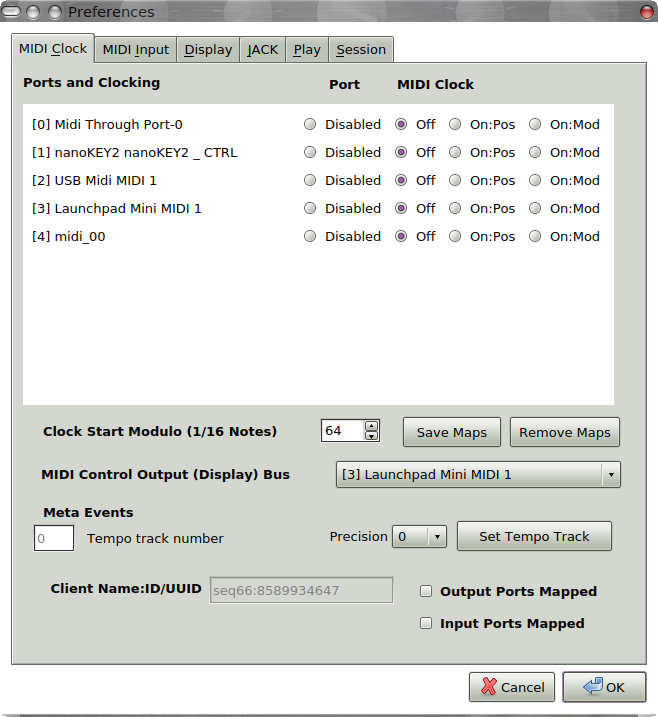
\includegraphics[scale=0.75]{main-menu/edit/preferences/midi_clock_tab.png}
   \caption{MIDI Clock Tab, ALSA Devices}
   \label{fig:midi_clock_tab}
\end{figure}

   The following elements are present in this tab:

   \begin{enumber}
      \item \textbf{Ports and Clocks Table}
      \item \textbf{Clock Start Modulo}
      \item \textbf{Save Clock/Input Maps}
      \item \textbf{Meta Events}
      \item \textbf{Client ID}
   \end{enumber}

   The \textbf{Ports and Clocks} table contains the following elements,
   although some can be removed by specifying the
   \texttt{port-naming = short} option in the 'rc' file.

   \begin{enumber}
      \item \textbf{Index Number}
      \item \textbf{Client Number}
      \item \textbf{Port Number}
      \item \textbf{Buss Name}
      \item \textbf{Port Disabled}
      \item \textbf{Off}
      \item \textbf{On (Pos)}
      \item \textbf{On (Mod)}
      \item \textbf{Clock Start Modulo}
   \end{enumber}

   The format of the left side of the entry listing is like the following:

   \begin{verbatim}
      [5] 128:4 yoshimi:input
       ^  ^   ^ ^
       |  |   | |
       |  |   |  -------- Buss name
       |  |    ---------- Port number
       |   ------------ Client number
        --------------- Index number
   \end{verbatim}

   \setcounter{ItemCounter}{0}      % Reset the ItemCounter for this list.

   \itempar{Index Number}{midi clock!index number}
   \index{index number}
   The number in square brackets is an ordinal indicating the position
   of the output buss in the list.
   For all practical purposes in \textsl{Seq66}, it \textsl{is} the
   buss/port number.  This number can be stored in a pattern in order to have
   the pattern's output go to that buss.  
   This is true even if port-mapping is in place.
   \index{port!mapping}
   \index{buss!mapping}
   \index{port!override}
   \index{buss!override}
   It can be used with the \texttt{-b},
   \texttt{-{}-buss}, or \texttt{ -{}-bus} options to redirect all
   pattern output to that buss, useful if only one buss is active or the
   \textsl{Seq66} patterns route to non-existent busses.

   \itempar{Client Number}{midi clock!client number}
   \index{client number}
   The number that precedes the colon is the "client number".
   It is useful mainly in ALSA, where clients can have numbers like "14",
   "128", "129", etc.  For native JACK mode, it matches the index number or is
   the name of the client (e.g. "seq66").

   \itempar{Port Number}{midi clock!port number}
   \index{port number}
   The number that follows the colon is the "port number".
   It is useful mainly in ALSA.
   For native JACK mode, it matches the index number.

   \itempar{Buss Name}{midi clock!buss name}
   \index{port name}
   \index{midi clock!port name}
   These labels indicate the output busses (ports) available.
   \textsl{Seq66} does not access devices by name, but by port number.
   However, a port-map can be created to make it possible to find the correct
   buss / port number by name lookup.

   \itempar{Port Disabled}{midi clock!port disabled}
   The \textbf{Port Disabled} clock choice marks an output port
   that the user does not want to use or that the operating system
   (\textsl{Windows} \smiley)
   is locking or disabling.
   Normally, this inaccessible port would cause \textsl{Seq66} to exit.
   With the port disabled, the inaccessible port is ignored.
   This feature also shows when a port-map cannot find a device in the system's
   device list.
   When the \textsl{Windows} version of \textsl{Seq66}
   (\texttt{qpseq66.exe}) is first started, it may error out.
   It will then write \texttt{erroneous.rc}
   and \texttt{erroneous.usr} configuration
   files, which can be examined to find the offending buss, which can then be
   marked in the normal 'rc' file as disabled.

   \itempar{Off}{midi clock!off}
   Disables the MIDI \textsl{clock} for the given output buss.
   MIDI output is still sent to those ports, and
   each port that has a device connected to it will play music.
   Some synthesizers may require this setting.

   \itempar{On (Pos)}{midi clock!on (pos)}
   MIDI clock will be sent to this buss.
   MIDI Song Position and MIDI Continue will be sent if playback starts
   at greater than tick 0 in Song mode.  Otherwise, MIDI Start will be sent.

   \itempar{On (Mod)}{midi clock!on (mod)}
   MIDI clock will be sent to this buss.
   MIDI Start will be sent, and clocking will begin
   once the Song Position has reached the start modulo of the specified size
   (see the next item's description).
   This setting is used for gear that does not respond to Song Position.

   Below the \textbf{Ports and Clocks Table} are more configuration elements.

   \setcounter{ItemCounter}{0}      % Reset the ItemCounter for this list.

   \itempar{Clock Start Modulo}{midi clock!clock start modulo}
   Clock Start Modulo (1/16 Notes).
   This value starts at 1 and ranges up to 16384, and defaults to 64.
   It is used by the \textbf{On (Mod)} setting discussed above.
   It is the \texttt{[midi-clock-mod-ticks]} option in the \textsl{Seq66}
   'rc' file.

   \itempar{Save Clock/Input Maps}{midi clock!port mapping}
   \index{port mapping}
   \index{port!mapping}
   Pressing this button saves the current set of MIDI I/O ports to sections in
   the 'rc' file.  These sections can be enabled in order to support
   port-mapping in subsequent runs of \textsl{Seq66}.

   \itempar{Meta Events}{midi clock!meta events}
   \index{tempo-track-number}
   This section consists of one item, the Tempo Track number.
   It allows the user to move the tempo track from pattern 0 to
   another pattern.  Changing this option is not recommended, since track 1 (0)
   is the official track for tempo events, but \textsl{Seq66} allows the
   user to record tempo events to another track.  \textsl{Seq66} will
   process tempo events in any pattern.
   \textsl{The "Set as Tempo Track" button to the right is not yet functional.}

   \itempar{Seq66 Client ID}{client ID}
   This read-only text field shows the client ID number assigned to
   \textsl{Seq66} by the ALSA MIDI subsystem.

   \itempar{Output Ports Mapped}{mapping}
   This read-only check-box shows if the port-mapper is active for the output
   ports.  This item can only be edited by closing the application, editing the
   'rc' file, and restarting the application.

   \index{todo!manual alsa gui option}
   There is currently no user-interface item corresponding to the "manual-ports"
   command-line and 'rc' configuration file option.
   We should rename this option to "virtual" eventually.

\paragraph{Menu / Edit / Preferences / MIDI Input}
\label{paragraph:menu_edit_preferences_midi_input}

   To set up \textsl{Seq66} to record MIDI from devices such as
   controllers and keyboards, the output of the ALSA MIDI recording
   command-line \texttt{arecordmidi -l} is relevant.
   Something like that listing appears in the Input tab:

\begin{figure}[H]
   \centering 
   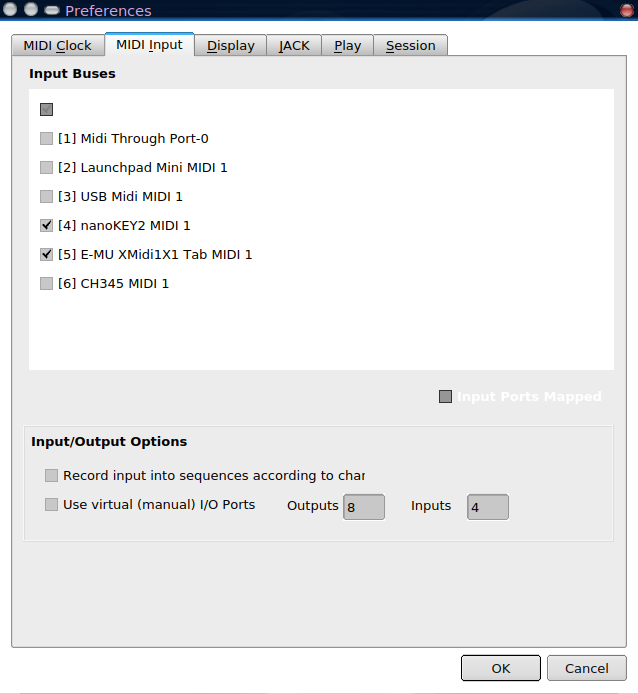
\includegraphics[scale=0.75]{main-menu/edit/preferences/midi_input_tab.png}
   \caption{MIDI Input, ALSA View}
   \label{fig:midi_input_tab}
\end{figure}

   Any item checked allows \textsl{Seq66} to record MIDI from that source,
   which must be connected to this input port.

   \textbf{Warning:}
   \index{warnings!usr config}
   \index{usr config}
   If the 
   \texttt{[user-midi-bus-definitions]} value in the 'usr' configuration file
   is non-zero, and the
   corresponding number of
   \texttt{[user-midi-bus-N]} settings are provided, then
   the list of existing hardware will be ignored, and those values will be
   shown instead.
   This feature can be overridden with the
   \texttt{-{}-reveal-ports} (\texttt{-r}) option.
   If you define these sections, they should match your
   hardware exactly, and your hardware should not change from session to
   session.

   If the "auto ALSA ports" option is turned on, via the \texttt{-a} or
   \texttt{-{}-auto-ports} option, then
   the input ports from the system are shown.

   \setcounter{ItemCounter}{0}      % Reset the ItemCounter for this list.

   \itempar{Input Buses}{input buses}
   \textbf{Input Buses} delineates the MIDI input devices as noted above.

   \itempar{Input Options}{input options}
   \index{input options}
   \textbf{Input Options} adds further refinements to MIDI input.
   Currenty it has only one setting, for recording input into patterns by the
   channel in each event.

   \itempar{Input Ports Mapped}{mapping}
   This stand-alone
   read-only check-box shows if the port-mapper is active for the input
   ports.  This item can only be modified by closing the application, editing
   the 'rc' file, and restarting the application.

   \itempar{Input Option}{input options}
   \index{input by channel}
   \textbf{Record input into sequence according to channel}
   causes MIDI input with multiple channels to be distributed to
   each sequence according to MIDI channel number.
   When disabled, the normal recording behavior dumps all data into the current
   sequence, regardless of channel.

\paragraph{Menu / Edit / Preferences / Keyboard (Removed)}
\label{paragraph:menu_edit_preferences_keyboard}

   The default keyboard mappings follow \textsl{Seq24} fairly well,
   but add a large number of additional controls.
   \textsl{Seq66} does not provide a user-interface to edit
   control keystrokes; around 96 keystroke slots would need to be provided!
   The keystroke and MIDI controls are consolidated, and are easy to change by
   editing the appropriate 'ctrl' configuration file, stored in one of the
   following directories, depending on
   the operating system:
   
   \begin{verbatim}
         /home/username/.config/seq66/qseq66.ctrl           (Linux)
         C:/Users/username/AppData/Local/seq66/qpseq66.ctrl (Windows)
   \end{verbatim}

   There are also some extended example present in the \textsl{Seq66}
   \texttt{data/linux} directory.

   For more information on keystrokes, see
   \sectionref{subsec:kbd_mouse_keyboard_control}.

\paragraph{Menu / Edit / Preferences / Mouse (Removed)}
\label{paragraph:menu_edit_preferences_mouse}

   This item selected the mouse-interaction method.
   It is not supported in \textsl{Seq66}...
   the "Fruity" interaction method is not available.
 
\paragraph{Menu / Edit / Preferences / Display}
\label{paragraph:menu_edit_preferences_display}

   This dialog provides a few odds and ends to enhance the user-interface.
   Some of these items (plus a few more) can be configured by editing the 'usr'
   file.

\begin{figure}[H]
   \centering 
   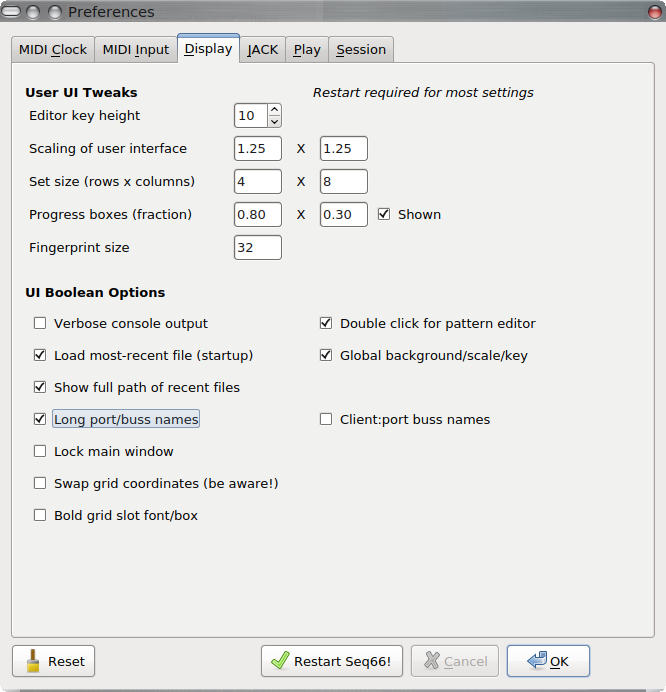
\includegraphics[scale=0.75]{main-menu/edit/preferences/midi_display_tab.png}
   \caption{Display Options}
   \label{fig:midi_display_tab}
\end{figure}

   \setcounter{ItemCounter}{0}      % Reset the ItemCounter for this list.

   \itempar{Editor Key Height}{key height}
   This option affects the pattern editor's piano roll.  Smaller means a wider
   range of notes can be shown.  It might be a good idea at some point to
   implement a vertical zoom.

   \itempar{Scaling of User Interface}{window scaling}
   These two items set scale factor for width and height of the main window.
   The lowest scale factor is 0.5, and the largest scale factor is 3.0.
   For the smallest window, the smallest practical values are 0.85 x 0.60.

   \itempar{Palette File Base Name}{palette}
   This text edit holds the base name of a 'palette' file, which is always
   stored in the \textsl{Seq66} configuration directory.

   \itempar{Save Current Palette}{palette}
   Normally, there is no palette file.  Pushing this button creates one, which
   can then be modified and configured as the palette-file to use in the 'rc'
   file.
 
\paragraph{Menu / Edit / Preferences / JACK}
\label{paragraph:menu_edit_preferences_jack}

   This tab sets up JACK transport, if \textsl{Seq66}
   was built with JACK support.
%  It now also supports native JACK MIDI.
   This tab also sets up options for using LASH session management, \textsl{if}
   \textsl{Seq66} was built with LASH support, which is no longer the
   default, even though it is shown in the figure below.

\begin{figure}[H]
   \centering 
   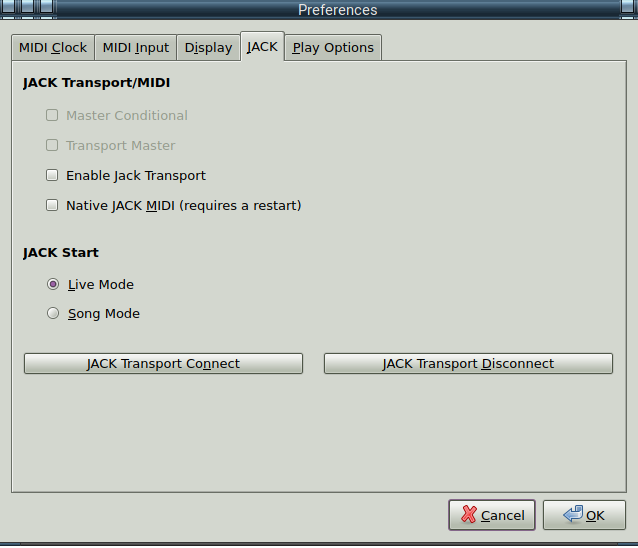
\includegraphics[scale=0.75]{main-menu/edit/preferences/midi_jack_tab.png}
   \caption{File / Options / JACK}
   \label{fig:menu_edit_preferences_jack_sync}
\end{figure}

   The main sections in this dialog are:

   \begin{enumber}
      \item \textbf{JACK Transport/MIDI}
      \item \textbf{JACK Start Mode}
      \item \textbf{JACK Transport Connect and Disconnect}
      \item \textbf{LASH Options}
   \end{enumber}

   \setcounter{ItemCounter}{0}      % Reset the ItemCounter for this list.

   \itempar{Transport/MIDI}{jack sync!transport/midi}
   These settings are stored in the 'rc' file settings group
   \texttt{[jack-transport]}.
   This items collects the following settings:

   \begin{itemize}
      \item \textbf{Jack Transport}.
         \index{JACK!transport}
         Enables slave synchronization with JACK Transport.
         The command-line option is \texttt{-{}-jack-transport}.
         The behavior of this mode of operation is perhaps not quite
         correct.  Even as a slave, \textsl{Seq66} can start and
         stop playback.
         Note that this option cannot be disabled via the mouse if the
         \textbf{Transport Master} option is enabled.  Disable that one first.
      \item \textbf{Transport Master}.
         \index{JACK!transport master}
         \textsl{Seq66} will attempt to serve as the JACK Master.
         The command-line option is \texttt{-{}-jack-master}.
         \textbf{Tip}:
         \textsl{Seq66} generally works better as JACK Master.
         If this option is enabled the \textbf{JACK Transport} option is
         automatically enabled as well.
      \item \textbf{Master Conditional}.
         \index{JACK!master conditional}
         \textsl{Seq66} will fail to serve as the JACK Master if there is
         already a Master.
         The command-line option is \texttt{-{}-jack-master-cond}.
         If this option is enabled the \textbf{JACK Transport} option is
         automatically enabled as well.
      \item \textbf{Native JACK MIDI}.
         \index{JACK!native midi}
         This option is for the \texttt{seq66} version of
         \textsl{Seq66}.
         If set, MIDI input and output use native JACK MIDI,
         rather than ALSA.  However, if JACK is not running on the
         system, then \texttt{seq66} will fall back to ALSA mode.
         The command-line option is \texttt{-{}-jack-midi}.
   \end{itemize}

%  Note that there are long-standing issues with the JACK support of
%  \textsl{Seq24}, and \textsl{Seq66} currently inherits some of them,
%  in spite of some bug fixes.  Generally, if one experiences issues in
%  transport control, try making one of the other sequencer applications the
%  JACK Master.
%  If one starts \textsl{Seq66} in JACK mode without JACK running,
%  it will take a little while for \textsl{Seq66} to start up, and it
%  will fall back to ALSA usage.

   If one makes a change in the JACK transport settings, it is best to
   then press the \textbf{JACK Transport Disconnect} button, then the
   \textbf{JACK Transport Connect} button.  Another option is to restart
   \textsl{Seq66}... the settings are automatically saved when
   \textsl{Seq66} exits.

   \itempar{JACK Start mode}{jack sync!start mode}
   This item collects the following settings, also stored in the 'rc' file
   settings group \texttt{[jack-transport]}.

   \begin{itemize}
      \item \textbf{Live Mode}.
         \index{JACK!live mode}
         \index{live mode}
         \index{non-playback mode}
         Playback will be in live mode.  Use this option to allow muting and
         unmuting of patterns.  This option might also be called "non-song
         mode".
         The command-line option is \texttt{-{}-jack-start-mode 0}.
      \item \textbf{Song Mode}.
         \index{JACK!song mode}
         \index{song mode}
         \index{playback mode}
         \index{performance mode}
         Playback will use only the Song Editor's data.
         The command-line option is \texttt{-{}-jack-start-mode 1}.
   \end{itemize}

   \textsl{Seq66} also selects the playback modes
   according to which window started the playback.
   \textsl{The main window}, or pattern
   window, causes playback to be in live mode.  The user can arm and mute
   patterns in the main window by clicking on sequences, using their hot-keys,
   and by using the group-mode and learn-mode features.
   The song editor causes playback to be in performance mode, also known as
   "playback mode", or \textbf{Song} mode.

   \itempar{Connect}{jack sync!connect}
   Connect to JACK Sync.
   This button is useful to restart JACK sync when making changes to it,
   or when \textsl{Seq66} was started in ALSA mode.

   \itempar{Disconnect}{jack sync!disconnect}
   Disconnect from JACK Sync.
   This button is useful to stop JACK sync when making changes to it.

   \itempar{LASH Options}{lash!option}
   Currently contains only one item, which enables the usage of LASH session
   management.  Currently, \textsl{Seq66} needs to be restarted to
   complete the enabling or disabling of LASH support.  Like the rest of the
   options, this one is written to the 'rc' configuration file.
   However, LASH is no longer supported in the default build.

   JACK connection and disconnection are disabled during playback, but the
   buttons don't yet reflect that status.

\paragraph{Menu / Edit / Preferences / Play Options}
\label{paragraph:menu_edit_preferences_play_options}

   There is currently only one setting in this tab:

   \textbf{Resume Note Ons at start/stop or sequence toggle}.
   This option allows notes that had already started
   to be resumed when playback resumes.

\subsection{Menu / Help / About...}
\label{subsec:menu_about}

   This menu entry shows the "About" dialog.
   That dialog provides access to some credits for the program as well.
   authors and the project documentors.
   It also shows Git version-control information as well.

\subsection{Menu / Help / Build Info...}
\label{subsec:menu_build_info}

   This menu entry shows the "Build Info" dialog.  This list of
   build options enabled in the current application is the same list
   that it generated via this command line:

   \begin{verbatim}
      $ seq66 --version
   \end{verbatim}

%-------------------------------------------------------------------------------
% vim: ts=3 sw=3 et ft=tex
%-------------------------------------------------------------------------------
